\begin{appendices}

\chapter{Terminology}

Traffic control engineering involves specific terminology to refer to different signal controls, timing plans, and controller types. This section offers a brief introduction of traffic signal control and terminology that may be used throughout the remainder of this report.

Modern intersections with traffic signals are controlled by a roadside \emph{signal controller}. Controllers switch power to signal lanterns and determine the sequence of display for each set of lights, operating under the safety requirement that no two conflicting flows receive green signals simultaneously. A typical controller operates lights in sequences called \emph{phases}, which are dynamic length allocations of green light time to a set of non-conflicting flows at an intersection. Typically, modern controllers include the following fixed or dynamic time allocations within a phase:

\begin{itemize}
\item \emph{late start time}, a fixed length of time a green light may be delayed for safety of other movements (e.g. pedestrian protection)
\item \emph{minimum green time}, a fixed length of time that a phase must operate before changing
\item \emph{inter-green time}, a fixed length of time required to operate amber and red signals at the end of a phase, typically at least 6 seconds. 
\item \emph{extension green time}, a dynamic length of time allocated to a phase determined after all required fixed times have been deducted from the total phase tie. 
\item \emph{maximum green time}, if the addition of the previous four time allocations exceeds the fixed maximum green time the phase is forced to change. 
\end{itemize}

A \emph{cycle} (or \emph{plan}) is an ordered sequence of one or more phases which is repeated by a controller. A fixed cycle traffic controller runs each phase for a fixed length of time within a static cycle. An actuated traffic controller can respond to sensor inputs from lane road loops and skip phases that are not in demand. Adaptive traffic controllers differ in implementation but typically can extend or shorten the length of a phase if a queue is completely cleared midway through a phase. The length of a cycle of an adaptive controller can be adapted to demand, typically running for a shorter length of time during quiet traffic and increasing in length to reduce queuing and satisfy high demand peaks \cite{scatstraining}.

An intersection has a given \emph{capacity}, defined as the maximum sustainable flow rate at which vehicles or pedestrians can travel through the intersection in a given time period. Capacity is dependant on the geometric layout of an intersection (e.g. width of road, number of lanes), driving and surface conditions, and traffic conditions. The \emph{degree of saturation} of an intersection is a ratio of arrival flow rate with respect to capacity of each approach for a given period. Arrival flow rate, also called \emph{demand flow}, refers to the number of vehicles or pedestrians arriving during a given period, measured from the back of a queue \cite{sidraglossary}. A section of road is said to be saturated if the traffic flow is equivalent to the capacity of the road at a given speed, such that any increase in flow will have a negative impact on the flow through the system. Any section of road where demanded traffic flow exceeds capacity is said to be \emph{congested} \cite{wallis2013costs}.


\chapter{SCATS Data File Format}

The following section contains an excerpt from a data file generated by the SCATS TrafficReporter application, and provided to this project by the Wellington City Council for research purposes. The data shown represents three cycles of SCATS operation at the intersection of Victoria Street and Vivian Street in Central Wellington, between 6:00AM and 6:02AM on the 20th June, 2013. An explanation of the format of the data is given below.

\begin{verbatim}
Thursday 20-June-2013 06:00 SS   3   PL 5.3  PVa3.3 CT   65 +0 RL 65, SA 10  DS 44
 Int   SA/LK    PH  PT!  DS  VO  VK!  DS  VO  VK!  DS  VO  VK!  DS  VO  VK! ADS
  520 S  10  '   A  36!  64  10  10!  57   9  10!   -       -!   -       -!   44
  520 S  11 ^    2  26!  17   2   2!   0   0   0!   -       -!   -       -!   19
  530 S  12 *'   A  35!  57   9   8!  41   7   6!   -       -!   -       -!   35
  530 S  13      B  24!  30   4   3!  16   2   2!  15   2   2!   -       -!   14
  520 S 273 ^    B  26!  17   2   2!   -       -!   -       -!   -       -!   23
A=<65>  B=35
Thursday 20-June-2013 06:01 SS   3   PL 5.3  PVa2.3 CT   65 +0 RL 65, SA 10  DS 54
 Int   SA/LK    PH  PT!  DS  VO  VK!  DS  VO  VK!  DS  VO  VK!  DS  VO  VK! ADS
  520 S  10  '   A  41!  43   8   7!  55  11  11!   -       -!   -       -!   54
  520 S  11 ^    2  25!  14   2   2!  56   4   6!   -       -!   -       -!   36
  530 S  12 *'   A  67!  26   8   7!  36  11  10!   -       -!   -       -!   40
  530 S  13      B   0!   0   0   0!   0   0   0!   0   0   0!   -       -!   10
  520 S 273 ^    B  25!   0   0   0!   -       -!   -       -!   -       -!   13
A=<64>  B=36
Thursday 20-June-2013 06:02 SS   3   PL 5.3  PV 0.3 CT   65 +0 RL 65, SA 10  DS 44
 Int   SA/LK    PH  PT!  DS  VO  VK!  DS  VO  VK!  DS  VO  VK!  DS  VO  VK! ADS
  520 S  10  '   A  65!  27   9   7!  21   8   6!   -       -!   -       -!   44
  520 S  11 ^    2   0!   0   0   0!   0   0   0!   -       -!   -       -!   22
  530 S  12 *'   A  41!  12   3   2!  34   7   6!   -       -!   -       -!   40
  530 S  13      B  23!  11   2   1!   0   0   0!   0   0   0!   -       -!   12
  520 S 273 ^    B   0!   0   0   0!   -       -!   -       -!   -       -!    4
A=<64>  B=36
\end{verbatim}

\begin{itemize}
\item \textbf{PT!} Phase time
\item \textbf{DS} Degree of Saturation
\item \textbf{V0} Vehicle actuations
\end{itemize}

\chapter{SCATS Intersection Configurations}
\label{appendix:scats_intersections}

Figure ~\ref{scats_intersections} shows three evaluation intersections used during the experimentation procedure as represented in the SCATS system used by Wellington City Council. Screenshots were provided by Wellington City Council traffic engineers.

\begin{figure}[H]
\centering
\begin{subfigure}{.5\textwidth}
  \centering
  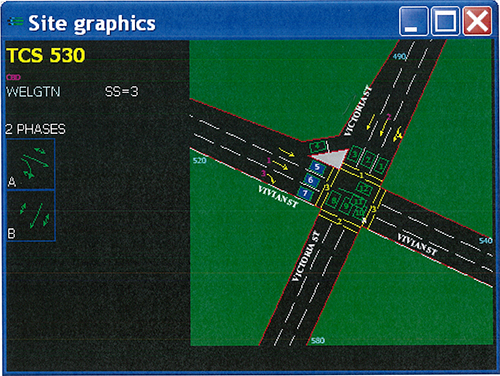
\includegraphics[scale=0.35]{scats-vivian-victoria.png}
  \caption{Vivian Street-Victoria Street}
  \label{fig:sub1}
\end{subfigure}%
\begin{subfigure}{.5\textwidth}
  \centering
  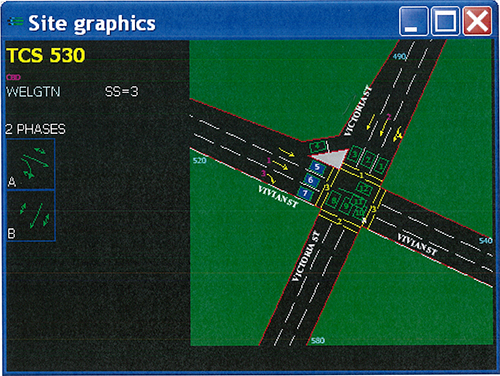
\includegraphics[scale=0.35]{scats-vivian-victoria.png}
  \caption{Courtenay Place-Tory Street}
  \label{fig:sub2}
\end{subfigure}

\vspace{1cm}

\begin{subfigure}{.5\textwidth}
  \centering
  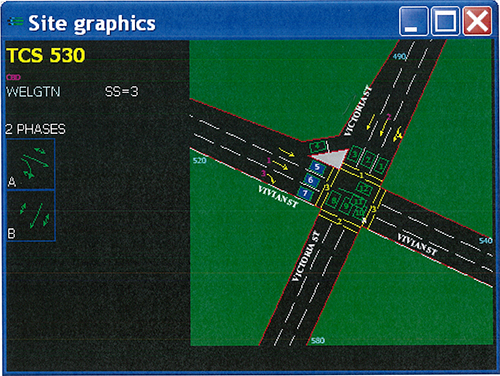
\includegraphics[scale=0.35]{scats-vivian-victoria.png}
  \caption{Karo Drive-Victoria Street}
  \label{fig:sub1}
\end{subfigure}%
\caption{ Intersections of Vivian-Victoria, Courtenay-Tory, and Karo-Victoria as represented in the SCATS system. }
\label{scats_intersections}
\end{figure}

\end{appendices}
